Rajapinnat mahdollistavat tiedonvaihdon eri järjestelmien ja toimijoiden välillä. Ne voivat olla standardissa määriteltyjä, eri abstraktiotasoille ja osittain toistensa päälle rakentuvia, tai hyvin suljettuja laitteen valmistajan kehittämiä. Lisäksi yhtenä rajapintana lämpöpumpuille ja aurinkoinverttereille voidaan ajatella AMI-mittareita.

Valmistajan tarjoamat pilvipalvelut toimivat rajapintana järjestelmän etähallintaan ja\linebreak -monitorointiin omistajalle. Myös valmistaja itse voi hyödyntää tätä rajapintaa esimerkiksi selvittämällä etänä laitteistovikaa tai keräämällä tilastoja järjestelmän toimivuudesta. Teknisesti ajatellen pilvipalvelu on kuitenkin standardoimaton, valmistajan itse kehittämä, joten tekninen toteutus on piilotettu. Tämän vuoksi tässä kappaleessa ei perehdytä tarkemmin pilvipalveluun, vaan se esitellään vain yleisesti.

Kaikkein matalimman abstraktiotason rajapintoja eli fyysisiä liitäntöjä tai sarjaliikenneprotokollia ei tässä työssä käsitellä tarkemmin. Tässä kappaleessa on kuvattu eri standardeissa määriteltyjen rajapintojen toimintaa ja käyttötarkoituksia. Lisäksi tarkastellaan myös \gls{AMI}-mittareita rajapintana.

\section{Modbus}

  Modbus on automaatiossa käytetty palvelin--asiakas-mallin viestintäprotokolla. Sen on alun perin kehittänyt vuonna 1979 yritys nimeltään Modicon käytettäväksi valmistamiensa ohjelmoitavien logiikoiden eli \Gls{plc}:den väliseen viestintään. Nykyisin Modicon on osa ranskalaista Schneider Electriciä. Koska standardi on julkaistu avoimesti kaikkien käytettäväksi ja se on verrattain yksinkertainen, on se saavuttanut johtavan aseman teollisuudessa. Yleisimmille ohjelmointikielille on saatavilla Modbus-standardin toteuttavat kirjastot, joiden avulla voidaan ohjelmallisesti ohjata laitteita. Laajan levinneisyyden ansiosta Modbus soveltuu monien eri valmistajien laitteiden järjestelmien kanssa käytettäväksi. Teollisuuden lisäksi protokollaa käytetään myös talo- ja kiinteistöautomaatiossa. \mbox{\parencite{sousaPortugal, modbusAppSpec, modbusOrg}}

  Vuonna 2004 Schneider Electric siirsi standardin hallinnan voittoa tavoittelemattomalle Modbus-järjestölle\footnote{Modbus Organization, Inc}. Järjestön muodostavat automaatiolaitteita valmistavat yritykset ja yksittäiset henkilöt. Sen tehtäviin kuuluu ylläpitää ja kehittää Modbus-standardia ja siihen liittyviä dokumentteja sekä toimia etujärjestönä edistäen Modbusin käyttöä. Modbusiin liittyvien dokumenttien ja julkaisujen avulla edistetään eri valmistajien järjestelmien välistä kommunikaatiota ja helpotetaan niiden integraatioita toisiinsa. \parencite{modbusOrg}

  \subsection{Viestintä ja tietomalli}

  Modbus-protokollan toiminta perustuu palvelinlaitteella sijaitsevien muistialueiden lukemiseen ja kirjoittamiseen kuvassa \ref{fig:c_s} kuvatun asiakas--palvelin-mallin (client--server model, ennen tunnettu termillä master--slave model) mukaan.  Lukemalla tietoja asiakaslaite kykenee seuraamaan palvelinlaitteen tilaa ja kirjoittamalla ohjaamaan sen toimintaa. Tietojen lukeminen ja kirjoittaminen tapahtuu protokollan määrittämien kysely, vastaus- ja virheviestien perusteella. \parencite{modbusAppSpec}

  \begin{figure}[h]
    \centering
    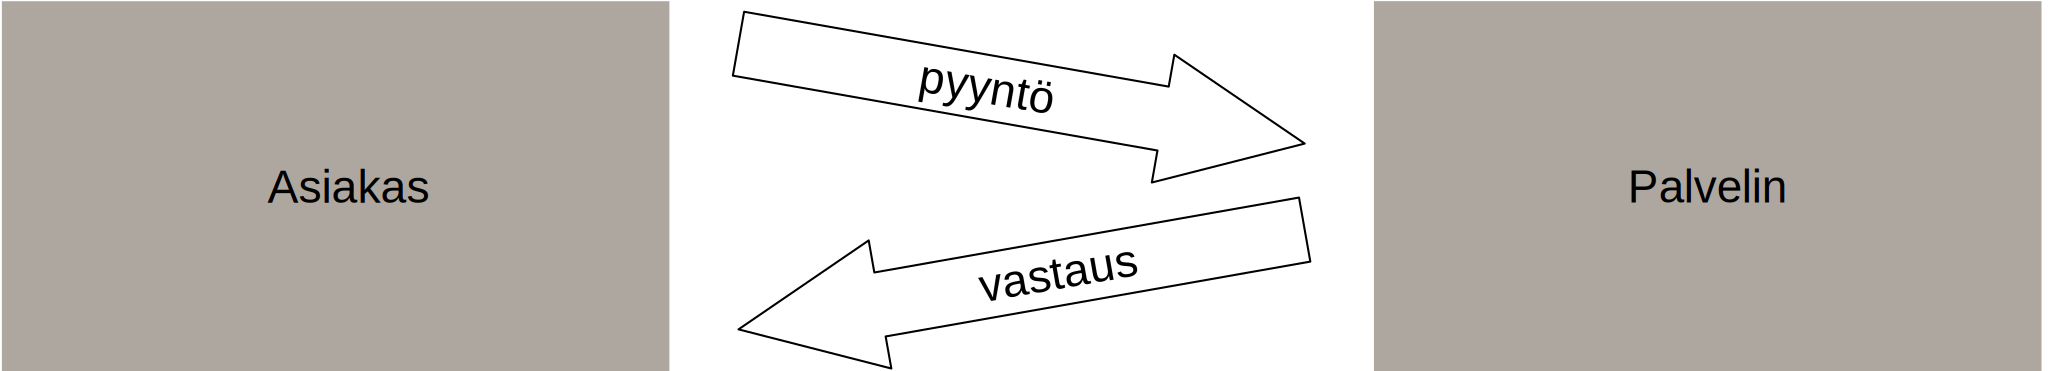
\includegraphics[width=1\textwidth]{figures/client_server}
    \caption[Asiakas--palvelin-malli]{Asiakas--palvelin-malli.  Perustuen lähteeseen \parencite{modbusAppSpec}}
    \label{fig:c_s}
  \end{figure}

  Modbus-verkko muodostuu yhdestä asiakkaasta, ja yhdestä tai useammasta palvelimesta. Palvelimet yksilöidään kokonaislukuosoitteella väliltä 1--247, mikä rajoittaa samaan verkkoon kytkettyjen latteiden määrää.  Protokolla rajoittaa kommunikointia niin, että kyselyitä lähettää vain asiakaslaite palvelinlaitteiden ainoastaan vastatessa niille osoitettuihin kyselyihin. \parencite{modbusSerialSpec} Tästä johtuen palvelinlaitteen eivät kykene itsenäisesti raportoimaan mahdollisesta virhetilanteesta tai tapahtumasta, vaan asiakaslaitteiden on jatkuvasti tehtävä kyselyitä pysyäkseen ajan tasalla. Tämä Modbusin ominaisuus vähentää sen käyttökelpoisuutta, varsinkin, mikäli kommunikointiresurssit ovat rajalliset.

  Modbus-protokolla määrittelee lähetettäville kyselyille kaksi eri muotoa: täsmälähetys (unicast) ja monilähetys (multicast). Täsmälähetys osoitetaan tietylle palvelimelle ja vastaanotettuaan sen palvelin toimii sen mukaisesti. Monilähetys taas lähetetään osoitteella~0, jolloin kaikki palvelimet reagoivat kyselyyn. \parencite{modbusSerialSpec} Kerrallaan vain yksi laite verkossa voi toimia asiakkaana muiden toimiessa palvelimina. Tästä huolimatta yksittäinen laite voi kuitenkin toimia sekä palvelimena, että asiakkaana, kunhan tämä tapahtuu erillisissä verkoissa. \parencite{DincerRosen}

  Modbus-protokollan tietomalli koostuu palvelinlaitteella sijaitsevista muistialueista, jotka on jaettu taulukoihin. Pääasialliset neljä muistialuetaulukkoa on kuvattu taulukossa \ref{taulukot}. Taulukoiden nimeäminen suomen kielellä on haastavaa, joten se jätetään tekemättä.
  \begin{table}[h]
    \centering
    \caption[Modbus muistialuetaulukot.]{Modbus muistialuetaulukot. Perustuu lähteeseen \parencite{modbusAppSpec}.}
    \begin{tabular}{|l|l|l|}
      \hline
      \rowcolor{gray} taulukon tyyppi         & datatyyppi      & asiakkaan oikeudet  \\ \hline
      \cellcolor{lightgray}Discretes Input    & 1 bitti          & vain luku           \\ \hline
      \cellcolor{lightgray}Coils              & 1 bitti          & luku/kirjoitus      \\ \hline
      \cellcolor{lightgray}Input Registers    & 16-bittinen sana & vain luku           \\ \hline
      \cellcolor{lightgray}Holding Registers  & 16-bittinen sana & luku/kirjoitus      \\ \hline
    \end{tabular}
    \label{taulukot}
  \end{table}
  1-bittisiä muistipaikkoja voidaan käyttää esimerkiksi päälläolotietojen välittämiseen, kun taas kahden tavun mittaisia muistipaikkoja voidaan käyttää esimerkiksi mitattujen arvojen ilmoittamiseen. Protokolla ei kuitenkaan määritä miten muistipaikkoja kuuluu käyttää, vaan tämä jätetään sovelluksen tekijän päätettäväksi. Kussakin taulukossa on 65536 erillistä osoitetta, joihin dataa voi tallentaa. Datan käsittely tapahtuu joko yksittäisen osoitteen perusteella tai sitten useampi perättäinen osoite kerrallaan. \parencite{modbusAppSpec}

  \subsection{Protocol data unit}

    Laitteissa toimivien sovellusten väliseen tiedonsiirtoon käytetään \gls{PDU}:ta (Protocol Data Unit), joka koostuu funktiokoodista ja operaatioon tarvittavasta datasta. \gls{PDU}:ita on kolmenlaisia, ja ne on esitetty taulukossa \ref{pdu}.
    \begin{table}[h]
      \centering
      \caption[\gls{PDU}-tyypit.]{\gls{PDU}-tyypit. Perustuu lähteeseen \parencite{modbusAppSpec}.}
      \begin{tabular}{ccl}
      \cline{1-2}
      \multicolumn{1}{|c|}{\cellcolor[HTML]{5CB735}Funktiokoodi (F)}                & \multicolumn{1}{c|}{\cellcolor[HTML]{5CB735}Kyselyn data}    & Kysely-PDU   \\ \cline{1-2}
                                                                                    &                                                              &              \\ \cline{1-2}
      \multicolumn{1}{|c|}{\cellcolor[HTML]{5CB735}Funktiokoodi (F)}                & \multicolumn{1}{c|}{\cellcolor[HTML]{5CB735}Vastauksen data} & Vastaus-PDU  \\ \cline{1-2}
                                                                                    &                                                              &              \\ \cline{1-2}
      \multicolumn{1}{|c|}{\cellcolor[HTML]{D78989}Poikkeusfunktiokoodi (F + 0x80)} & \multicolumn{1}{c|}{\cellcolor[HTML]{D78989}Poikkeuskoodi}   & Poikkeus-PDU \\ \cline{1-2}
    \end{tabular}
      \label{pdu}
    \end{table}

    \gls{PDU}:n alun muodostaa funktiokoodi, joka on joko Modbus-protokollan tai käyttäjän määrittämä funktio. PDU:n loppuosa koostuu mahdollisesta datasta, jota palvelin tarvitsee suorittaakseen halutun toiminnon. Vastaus-PDU:hun tulee sama funktiokoodi kuin kysely-PDU:hun. Mikäli palvelin päätyy virhetilanteeseen, joko virheellisen kysely-PDU:n tai sisäisen virheen takia, vastaa se asiakkaalle poikkeus-PDU:lla, joka muodostuu funktiokoodista, johon on liitetty heksakoodi 0x80, ja poikkeuskoodista. \parencite{modbusAppSpec} Funktiokoodeista käytetyimmät liittyvät yksittäisten muistipaikkojen lukemiseen ja kirjoittamiseen \parencite{DincerRosen}. Lista yleisistä funktio- ja poikkeuskoodeista löytyy liitteestä \ref{app:modbus_funktio_koodit}.


  \subsection{Protokollan rakenne}

    Modbus-protokollasta on toteutettu muutamia eri versioita:
    \begin{itemize}
      \item sarjaväyläversio eli Modbus Serial, joka muodostuu kahdesta muunnelmasta:
      \begin{itemize}
        \item Modbus \gls{RTU} ja
        \item Modbus ASCII,
      \end{itemize}
      \item Modbus TCP/IP ja
      \item Modbus Plus.
      \parencite{modbusAppSpec}
    \end{itemize}
    Edellisistä Modbus Plus on Schneider Electricin hallinnoima, eikä se ole avoimesti saatavilla. Modbus Plus on oma Modbusista eroava standardinsa, jota ei tässä käsitellä enempää. \parencite{seCom}

    Taulukossa \ref{rakenne} on Modbus-protokollaperhettä verrattu \gls{OSI}-malliin. Modbus-protokollan ylempi kerros, eli \gls{MBAP} sijoittuu \gls{OSI}-mallissa kerroseen 7, eli sovelluskerrokseen. \gls{MBAP}:n toimintaa on esitelty edellisessä kappaleissa. Sarjaväyläversiossa alempi kerros sijoittuu \gls{OSI}-mallissa kerrokseen 2 ja Modbus TCP/IP:n tapauksessa kerrokseen 5\footnote{\gls{OSI}-mallin teoreettisesta luonteesta johtuen tästä voinee esittää eroavia mielipiteitä.}.
    \begin{table}
      \centering
      \caption[Modbus-protokollan rakenne, \gls{OSI}-malli ja SunSpec]{Modbus-protokolla ja  SunSpec Modbus suhteutettuna \gls{OSI}-malliin. Modbus-protokollaperhe sinisellä ja Sunspec Modbus keltaisella. Perustuu lähteisiin \parencite{osi, modbusSerialSpec, modbusTCPIPSpec, SSTech}.}
      \begin{tabular}{|c|c|ccc}
      \cline{1-2}
      \multicolumn{2}{|c|}{OSI-mali}                                               & \multicolumn{3}{c}{}                                                                                                                                                                \\ \hline
      \multicolumn{1}{|l|}{}                    &                                  & \multicolumn{3}{c|}{\cellcolor[HTML]{FFFFC7}SunSpec}                                                                                                                                \\ \cline{3-5}
      \multicolumn{1}{|l|}{\multirow{-2}{*}{7}} & \multirow{-2}{*}{sovelluskerros} & \multicolumn{3}{c|}{\cellcolor[HTML]{6F6FE6}\gls{MBAP} (Modbus-viestintäprotokolla)}                                                                                                      \\ \hline
      6                                         & esityskerros                     &                                                         &                                                           & \multicolumn{1}{c|}{}                                         \\ \cline{1-2} \cline{5-5}
      5                                         & istuntokerros                    &                                                         & \multicolumn{1}{c|}{}                                     & \multicolumn{1}{c|}{\cellcolor[HTML]{6F6FE6}Modbus-\gls{TCP}} \\ \cline{1-2} \cline{5-5}
      4                                         & kuljetuskerros                   &                                                         & \multicolumn{1}{c|}{}                                     & \multicolumn{1}{c|}{\gls{TCP}}                                \\ \cline{1-2} \cline{5-5}
      3                                         & verkkokerros                     &                                                         & \multicolumn{1}{c|}{}                                     & \multicolumn{1}{c|}{IP}                                       \\ \hline
      2                                         & siirtokerros                     & \multicolumn{1}{c|}{\cellcolor[HTML]{6F6FE6}Modbus-RTU} & \multicolumn{1}{c|}{\cellcolor[HTML]{6F6FE6}Modbus-ASCII} & \multicolumn{1}{c|}{Ethernet, ...}                            \\ \hline
      1                                         & fyysinen kerros                  & \multicolumn{2}{c|}{RS-232 / RS-485}                                                                                & \multicolumn{1}{c|}{Ethernet, ...}                            \\ \hline
      \end{tabular}
      \label{rakenne}
    \end{table}

    \gls{MBAP} on kaikille Modbus-versioille yhteinen ja se mahdollistaa viestinnän laitteiden kesken erilaisten verkkojen ylitse. Välitettävät funktiokoodit ja data pakataan \gls{MBAP}:n toimesta PDU:ksi. Alemmassa kerroksessa muodostetaan \gls{ADU}(application data unit), joka sisältää PDU:n lisäksi kohdelaitteen osoitteen ja tarkistussumman tai jos kyseessä on Modbus-TCP, \gls{MBAP}-otsikon. Erilaiset ADU:t on esitelty kuvassa \ref{fig:adu}.
    \begin{figure}[h]
      \centering
      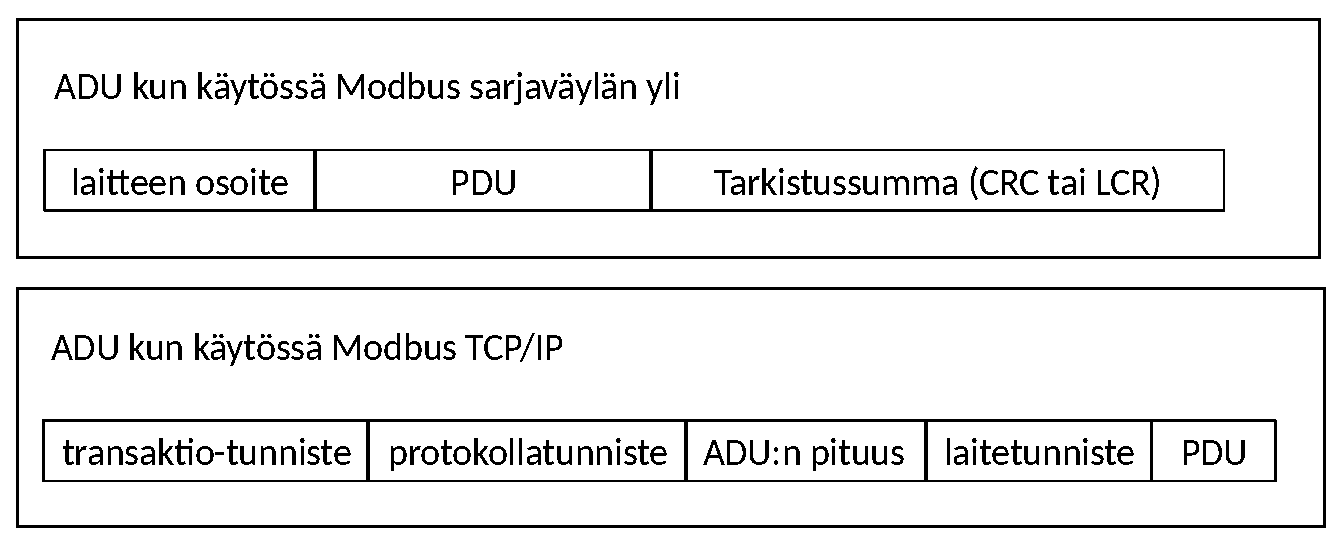
\includegraphics[width=1\textwidth]{figures/adu}
      \caption[ADU-tyypit]{Erilaiset ADU-tyypit.  Perustuen lähteisiin \parencite{modbusTCPIPSpec, modbusSerialSpec}}
      \label{fig:adu}
    \end{figure}

    Sarjaväylän yli toimivassa Modbusissa ADU siirretään käyttäen RS-485-standardia noudattavaa väylää tai RS-232-väylää pitkin. Oletuksena Modbus-standardi kehottaa laitevalmistajia toteuttamaan ainakin RS-485-rajapinnan, RS-232-rajapinnan ollessa vapaaehtoinen. Modbus \gls{RTU} siirtää datan suoraan bitteinä. Modbus \gls{ASCII}:ssa taas jokainen tavu koodataan kahdeksi heksadesimaalimerkiksi ennen lähetystä, mikä heikentää sen tiedonsiirtokykyä. Modbus-standardi edellyttää, että kaikki laitteet tukevat ainakin Modbus RTU:ta Modbus ASCII:n ollessa suositeltu. \parencite{modbusSerialSpec}

    Modbus TCP/IP:tä käytettäessä Modbus-liikenne voi kulkea normaalin Internet-liikenteen mukana, mikä tekee siitä hyvin joustavan ratkaisun. TCP-portti 502 on varattu Modbus-sovelluksille. \parencite{modbusTCPIPSpec} Koska ADU:t lähetetään TCP-kehyksessä, niihin ei tarvitse laskea eikä lisätä tarkistussummaa. TCP-protokolla huolehtii paketin (kehys + ADU) perille pääsystä ja mahdollisista uudelleenlähetyksistä. Tietosuojasta voidaan huolehtia käyttämällä kommunikointiin \gls{VPN}-yhteyttä. Toinen turvallisuutta parantava keino on käyttää kommunikointiin MODBUS/TCP Security -standardin mukaista TLS-salausta, jolloin liikenne kohdistetaan TCP-porttiin 802 \parencite{modbusTCPIPTLSSpec}.

\section{IEC 61850}
  \gls{IEC} 61850 on sähköaseman älykkäiden sähkölaitteiden kommunikaatioprotokollia määrittävä standardi. Se on laajasti käytössä sähköasemien tiedonvaihdossa ja sähkönjakelun automaatiossa. Sen laajennukset tähtäävät kuitenkin myös laajempaan käyttöön, sillä standardissa on määritelty myös esimerkiksi hajautetun energiantuotannon tietomalleja. Standardi määrittelee myös inverttereiden erilaisia toiminnallisuuksia, esimerkiksi:
    \begin{itemize}
      \item välittömät ohjaustoiminnot, esimerkiksi alasajo- ja käynnistyskomennot,
      \item loistehonsäädön (Volt/VAR-säätö) tilan muuttaminen,
      \item teho taajuuden funktiona -tilan muuttaminen (frequency-watt),
      \item toiminnan jatkaminen epätavallisista jännitevaihteluista huolimatta,
      \item normaalin toiminta-alueen määrittäminen ja irti kytkeytyminen sen ulkopuolella määritellyllä funktiolla,
      \item käyttäytymistilojen muuttaminen tehon funktiona,
      \item tehon muuttaminen jännitteen perusteella ja
      \item ajastetut komennot \parencite{61850funcs}.
    \end{itemize}

  IEC 61850 ei ole vielä laajasti käytössä inverttereissä, ja ainoa löydetty esimerkki sen suorasta käytöstä on SMA:n\footnote{SMA Solar Technology AG -- System-, Mess- und Anlagentechnik} tarjoama standardia hyödyntävä rajapinta Italiassa toimiville inverttereille \parencite{SMAManual}. Tällä voidaan irrottaa tai kytkeä invertteri verkkoon, tai muuttaa invertterin taajuusrajoja. Italian CEI 0-21 -standardissa vaaditaan inverttereille rajapinta verkonhaltijalle, jonka takia luultavasti tämä ominaisuus on SMA:n ohjekirjassa merkattu vain Italia -ominaisuudeksi. Tämän vaatimuksen\footnote{\url{http://blog.nettedautomation.com/2012/07/iec-61850-in-italy-sma-offers-iec-61850.html}} lähde ei ole alkuperäinen, joten tätä vaatimusta ei voitu vahvistaa varmaksi, tosin SMA:n erillinen ohjeistus Italian laitteille viittaa siihen.

  IEC standardin ja Modbusin välille on olemassa myös protokollamuuntimia, jolloin invertterit saadaan näkymään IEC standardin mukaisina laitteina. Esimerkiksi SMA:n keskusinvertterit voidaan liittää verkonhaltijan ohjaukseen erillisellä ohjauslaitteella, joka toimii samalla IEC61850-Modbus -muuntimena järjestelmälle, vaikka invertteri ei itsessään kyseistä standardia tuekaan \parencite{SMAPPManager}. Tämä toteuttaa silloin Fingridin VJV2018 -dokumentissa määritellyt etäohjausvalmiusvaatimukset yli \SI{1}{\mega\watt}:n suuruisille voimalaitoksille \parencite{VJV2018}.

\section{SunSpec Modbus}
  SunSpec Modbus on SunSpec Alliancen määrittelemä sovellustason toteutus, joka hyödyntää yleisesti käytössä olevaa Modbus-protokollaa. Sunspec Modbus sijoittuu rakenteellisesti Modbusin päälle, kuten taulukossa 4.3 kuvattiin. Fyysinen Modbus-rajapinta on sisäänrakennettu noin \SI{80}{\percent}:iin asennetuista hajautetun energiantuotannon laitteista, joten tämän toteutuksen tuominen suurelle määrälle laitteita on melko yksinkertaista \parencite{SSFactSheet}.

  SunSpecin standardi on tehty huomioiden \gls{IEC} 61850 -standardi, mukaan lukien sen 90-7 ja 7-420 -laajennukset, jotka käsittelevät hajautetun energiantuotannon inverttereiden ja konverttereiden toiminnallisuuksia ja kommunikaatiorakennetta hajautetussa energiantuotannossa. SunSpec onkin toteuttanut edellä mainitut toiminnallisuudet myös omaan standardiinsa. Tämän tarkoituksena on helpottaa integraatiota \gls{IEC} 61850 -standardia hyödyntävien järjestelmien kanssa \parencite{SSTech}. Kuitenkaan SunSpec ei ole nimennyt tietomallin muuttujia täsmälleen samoilla nimillä, kuin 61850-standardi, joten ne eivät ole suoraan yhteensopivia keskenään.

  SunSpecin toteutuksessa on määritelty tietomalleja, joiden avulla eri valmistajien laitteita voidaan yhdistää samaan järjestelmään \parencite{SSTech}. Nämä tietomallit mahdollistavat laiteriippumattomuuden, sillä niissä on määritelty funktioiden toiminta ja niiden käyttö. Tällöin eri valmistajien laitteita voidaan lukea ja ohjata yhteisillä käskyillä järjestelmän sisällä.

  SunSpec Modbusin määrittelemät tietomallit ovat käytössä myös muilla protokollilla, kuten \gls{HTTP}/\gls{XML}:lla ja \gls{OPC}:lla \parencite{SSTech}. Koska lähes kaikki tieto SunSpecin standardista perustuu Modbus-protokollaan, muiden tiedonsiirtoprotokollien tarkastelu jätettiin pois. Tiedon puute johtuu mitä luultavimmin Modbusin hallitsevasta asemasta inverttereissä.

  SunSpec-protokollan yleisyys selvisi sähköpostikeskustelussa aurinkosähköjärjestelmiä Suomessa asentavan yrityksen kanssa. Solarigo Oy on asentanut järjestelmiä teholtaan noin sadasta kilowatista jopa 5,9 megawattiin. Se on käyttänyt viiden eri valmistajan aurinkoinverttereitä eri projekteissa, mutta useimmissa niistä ei ole tarvittu etä- tai paikallista ohjausta. Mikäli paikallista ohjausta on käytetty, kommunikaatio on toteutettu lähes poikkeuksetta RS-485 väylän kautta ja kaikissa tapauksissa SunSpecin protokollaan perustuen. Vaikka valmistajat ovat dokumentoineet, miten protokollalla ohjataan niiden laitteita, käytännön kokemus on osoittanut että kuitenkaan kaikki ominaisuudet eivät ole toimineet kuten ne on määritelty. \parencite{Solarigo}


\section{IEEE 1815 / Distributed Network Protocol 3}
  DNP3 on teollisuusautomaation kommunikaatioprotokolla, joka määriteltiin alun perin 1993 ja sen kehitys jatkuu edelleen. Vuonna 2008 yhdysvaltalainen valtionvirasto NIST ja voittoa tavoittelematon energia-alan järjestö \gls{EPRI} näkivät tarpeen rajapinnalle \gls{IEC} 61850:n ja DNP3:n välille. Koska DNP3 oli vain vakiintunut käytäntö, DNP3:n standardisointi oli tarpeen, jotta yhteistyö ja koordinointi \gls{IEC}:n kanssa olisi sujuvaa. DNP3 standardoitiinkin \gls{IEEE} 1815 -standardiksi vuonna 2010, jonka jälkeen siitä on käytetty tuota nimitystä \parencite{DNP3&61850}.

  DNP3 on suunnattu sähköteollisuuden käyttöön, mutta se on myös käytössä esimerkiksi energia- ja vesiteollisuudessa. Pohjois-Amerikassa DNP3 on käytössä sähköverkon \gls{SCADA}-järjestelmissä, ja se onkin osittain kilpaileva sähköasemastandardi IEC 61850:n kanssa.

  IEEE 1815.1 -dokumentti määrittelee standardisoidun tavan linkittää yhteen data tämän ja IEC-standardin välillä \parencite{IEEE1815.1}. Tämä mahdollistaa IEC 61850-standardia käyttävien laitteiden lisäyksen IEEE 1815-protokollaiseen järjestelmään. Tämän on Pohjois-Amerikassa tärkeää, sillä siellä on laajasti käytössä IEEE 1815 standardi, mutta koska IEC 61850 on ominaisuuksiltaan laajempi, sen osuus tulee kasvamaan. Molempien standardien kanssa työskentelevä Bruce Muschlitz arveli vuonna 2009 DNP3:n häviävän keskinäisen kilpailun, sillä IEC 61850 täyttää kaikkien sidosryhmien tarpeet ominaisuuksien puolesta \parencite{DNPvsIEC}. Tosin näiden kahden standardin yhteensovittaminen on muuttanut tilannetta, eikä DNP3 tule välttämättä häviämään markkinoilta vielä pitkään aikaan, tosin automaatiolaitteiden elinikä on pitkä, joka vaikuttaa markkinajakaumaan ja uuden teknologian tuomiseen. 2019 tehdyn kyselyn mukaan DNP3:a käytti 94\% kyselyyn vastanneista sähköntuotanto ja -jakeluyrityksistä Pohjois-Amerikassa, mutta IEC 61850:n osuus on kasvamassa \parencite{DNP3Study}.

  Vuonna 2013 IEEE julkaisi dokumentin, joka auttaa verkonhaltijoita kommunikoimaan hajautetun energiantuotannon kanssa. Tämä dokumentti kuvaa standardoidun rajapinnan datalle ja joukon protokollapalveluita ja profiileja. Dokumentin kuvaamien profiilien tarkoitus on helpottaa hajautetun energiantuotannon liittämistä DNP3 järjestelmiin. Vuonna 2018 dokumenttia päivitettiin siten, että se lisäksi sisältää toiminnallisten ominaisuuden määrittelyt protokollalle, sekä linkityksen IEC-61850-7-420 tietomallin kanssa. Näiden uudistusten myötä DNP3 protokollaa voidaan käyttää älyinverttereiden ohjaukseen samalla tavalla kuin SunSpeciä tai IEC 61850-standardia, mutta myös käyttää näitä kolmea protokollaa rinnakkain toistensa kanssa. \parencite{DNP3Inv, DNP3AppNote}

  Vaikka DNP3 on standardoitu myös ohjaamaan aurinkoinverttereitä, valmistajat eivät ole ottaneet sitä käyttöön, ainakaan vielä. Sen toiminta on varmistettu tutkimuksissa, joissa on tehty testilaitteisto eri ohjaustoimintojen varmistamiseksi, mutta kaupallisista inverttereistä ei ole löytynyt mainintaa DNP3:n käytöstä. \parencite{DNP3Inv}


\section{Smart Grid -ready}

  Bundesverband Wärmepumpe e.V. (jäljempänä BWP) on saksalainen lämpöpuppuyhdistys, joka ylläpitää lämpöpumppujen ohjaukseen käytettävää rajapintaa määrittävää \gls{SG}-Ready-merkintää (\gls{SG} Ready label). \gls{SG}-Ready määrittelee pumpulle neljä eri toimintatilaa, joiden perusteella ulkoinen toimija kykenee ohjaamaan lämpöpumpun toimintaa. Toimintatilat yksi ja kaksi ovat yhteensopivia Saksassa käytetyn muun muassa lämpöpumppuihin kohdistetun energiantoimittajien suorittaman ohjauksen (EVU-Sperre\footnote{Energieversorgungsunternehmen Sperre}) kanssa.\parencite{SGReadyReg} Ohjattava lämpöpumppu voidaan kytkeä energiatoimittajan toimesta pois päältä enimmillään kahdeksi tunniksi kerrallaan. Yhteen vuorokauteen taas voi sijoittua enintään kolme keskeytystä, jotka on pyritään sijoittamaan suurimman kulutuksen hetkiin. Kun kuluttajan tekee sähkösopimuksen, johon ohjaus kuuluu, saa hän vastavuoroisesti alennusta energian hinnasta. \parencite{enwg, VDEARN4100}

  SG-Readyn  kolmas ja neljäs toimintatila ovat sopivia ylituotannon kompensointiin niiden lisätessä lämpöpumppujen sähkönkulutusta. Eri toimintatilat on eritelty taulukossa \ref{sgready}.
  \begin{table}[h]
    \centering
    \caption[\gls{SG}-Ready toimintatilat]{\gls{SG}-Ready toimintatilat. Perustuu lähteeseen \parencite{SGReadyReg}.}
    \begin{tabular}{|c|c|p{3in}|}
      \hline
      \rowcolor{lightgray} toimintatila & looginen kytkentä & kuvaus \\\hline
      1 & 1 0 & Lämpöpumppu on kytkettynä pois päältä. Enintään kaksi tuntia kerrallaan enintään kolme kertaa vuorokaudessa \\\hline
      2 & 0 0 & Normaali toimintatila. Varaudutaan mahdolliseen kahden tunnin pysäytykseen. \\\hline
      3 & 0 1 & Suositeltu päälläolo. \\ \hline
      4 & 1 1 & Pakotettu päälläolo. Mahdollisesti myös lisävastuksen pakotettu päälläolo. \\\hline
    \end{tabular}
    \label{sgready}
  \end{table}
  Jokaiselle toimintatilalle on määritelty binäärinen arvo (0b00 -- 0b11), joka voidaan toteuttaa kahdella loogisella tilalla. SG-Ready ei tarkemmin määrittele sitä, miten nämä tilat tuodaan ohjattavalle laitteelle. \parencite{SGReadyReg}

  SG-Ready on korkean abstraktiotason rajapinta, joka tarjoaa keinoja ohjausrajapintojen yhtenäistämiseen. Alemman tason kommunikointi, johon siis SG-Ready ei ota kantaa, pitää määritellä ja toteuttaa erikseen. Yksi alemman tason kommunikoinnissa yleisesti käytettävä standardi on Modbus-viestintäprotokolla.

\section{AMI-mittari}
  Verkonhaltijan omistamat sähkönkäyttöpaikkojen AMI-mittarit voivat toimia rajapintana lämpöpumpuille, ja tulevaisuudessa ehkä myös aurinkosähköjärjestelmille. Nykyään mittareissa tulee olla kuormanohjausrele, jota voidaan käyttää esimerkiksi 2-tariffiohjausta varten, jolloin lämmitys voidaan aktivoida yötariffin alkaessa ja lämmitys tapahtuu halvemmalla hinnalla \parencite{mittariAsetus}. Osassa mittareita on myös toinen ohjausrele jota voidaan hyödyntää tehonpudotukseen \parencite{kysJousto}. Lisäksi Suomessa noin 60\%:ssa sähkönkäyttöpaikoista on etäkatkaisu- ja kytkentäominaisuus, jolla voidaan katkaista sähköt koko sähkönkäyttöpaikasta. \parencite{AMRNykytila}

  Jo asennetuissa mittareissa voi olla luentarajapinta hetkelliselle kulutukselle, mutta se rajoittuu usein vain pulssilähdöksi \parencite{Aidon5510}. Esimerkiksi suomalaisen mittarivalmistaja Aidonin uudemmissa mittareissa on mahdollista lukea dataa \gls{HAN}-rajapinnasta, joka toimii M-bus-protokollan välityksellä käyttäen fyysisellä kerroksella \gls{8P8C}-liitintä. Rajapinnasta voi lukea esimerkiksi virta- ja jännitetietoja sekä tehotietoja verkosta mittarin suuntaan ja mittarista verkon suuntaan. \parencite{HAN, NVEHAN} Tätä voidaan hyödyntää kiinteistöautomaatiossa mittaritietona, jolloin asiakas voi kuluttaa kaiken tuottamansa energian sen verkkoon syöttämisen sijaan.

  AMI-mittaria voidaan tulevaisuudessa hyödyntää akullisissa aurinkosähköjärjestelmissä kuormanohjaukseen. Seuraavan sukupolven mittareihin voitaisiin lähettää tieto sähkön hinnasta, jolloin sähkönsyöttöä voidaan vaihtaa verkon ja energianvaraston välillä korkean hinnan aikaan. Älykäs mittarinluentajärjestelmä voi myös hyödyntää historiatietoja ja sääennustusta optimoidessa sähkövaraston käyttöä. Tällöin energiavarastoa voitaisiin varata yöllä halvemman sähkönhinnan aikaan, mutta varaaminen kuitenkin pääsääntöisesti tapahtuisi aurinkovoimalalla. \parencite{AMRNykytila}

  Keskeinen syy mittarien yksinkertaisiin kuormanohjauksiin on mittarin luotettavuus, sillä monimutkaisemmassa mittarissa on useampi hajoava komponentti. Myöskin mittareiden elinkaari on suhteellisen pitkä, 10--15 vuotta. Lisäksi verkonhaltijan saamat hyödyt ylimääräisistä rajapinnoista eivät ole suuret, ja uusien toiminnallisuuksien kehitys myöhäistäisi edelleen seuraavan sukupolven mittareiden asennusta. Lähtökohtaisesti tietoturvan ja kustannusten kannalta kannattavampaa onkin tarjota vain rajapinta mittarilta saatavalle tiedolle, kuten mittaukselle ja esimerkiksi energian hinnalle. Tällöin kiinteistöautomaatio voi hyödyntää näitä tietoja, ja siten hoitaa paikallisesti energiatasapainon optimointia.
